Là phương pháp mô hình hóa biến thiên 2D theo thời gian để phân tích chuỗi thời gian tổng quát. Hành động tách các khoảng thời gian khác nhau khỏi chuỗi thời gian có thể làm giảm đáng kể độ phức tạp để xử lý các mô hình. Ngoài ra, FFT (Fast Fourier Transform) giúp nắm bắt được sự thay đổi trong và giữa các thời kỳ. Quá trình này cho phép chuỗi thời gian được tách rời có cách diễn giải vật lý rõ ràng hơn, nâng cao khả năng diễn giải của mô hình.

\begin{figure}[htbp]
\centerline{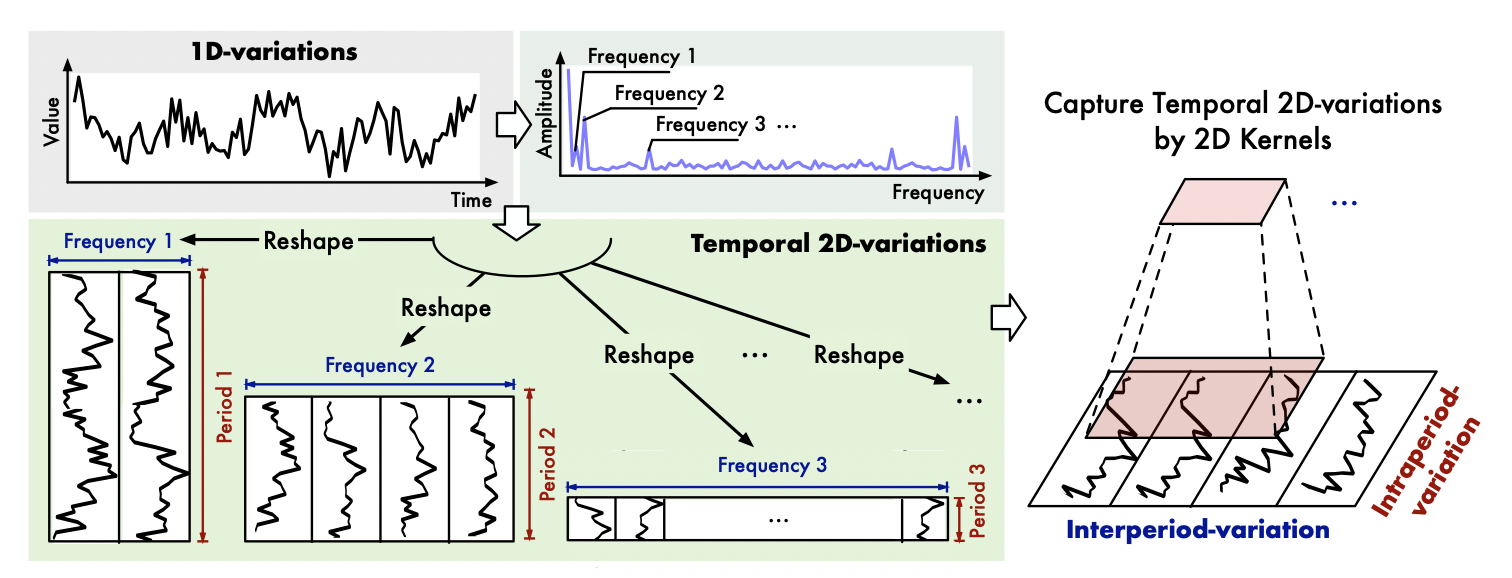
\includegraphics[width=0.4\textwidth]{img/2Dstructure.png}}
\caption{Minh họa cấu trúc 2D trong chuỗi thời gian.}
\label{fig}
\end{figure}

Bằng cách chuyển đổi dữ liệu chuỗi thời gian 1D thành một tập hợp các tensor 2D dựa trên nhiều chu kỳ, TimesNet phá vỡ giới hạn của chuỗi thời gian 1D và cho phép mô hình nắm bắt được sự biến đổi 2D theo thời gian của chuỗi thời gian.

\begin{figure}[htbp]
\centerline{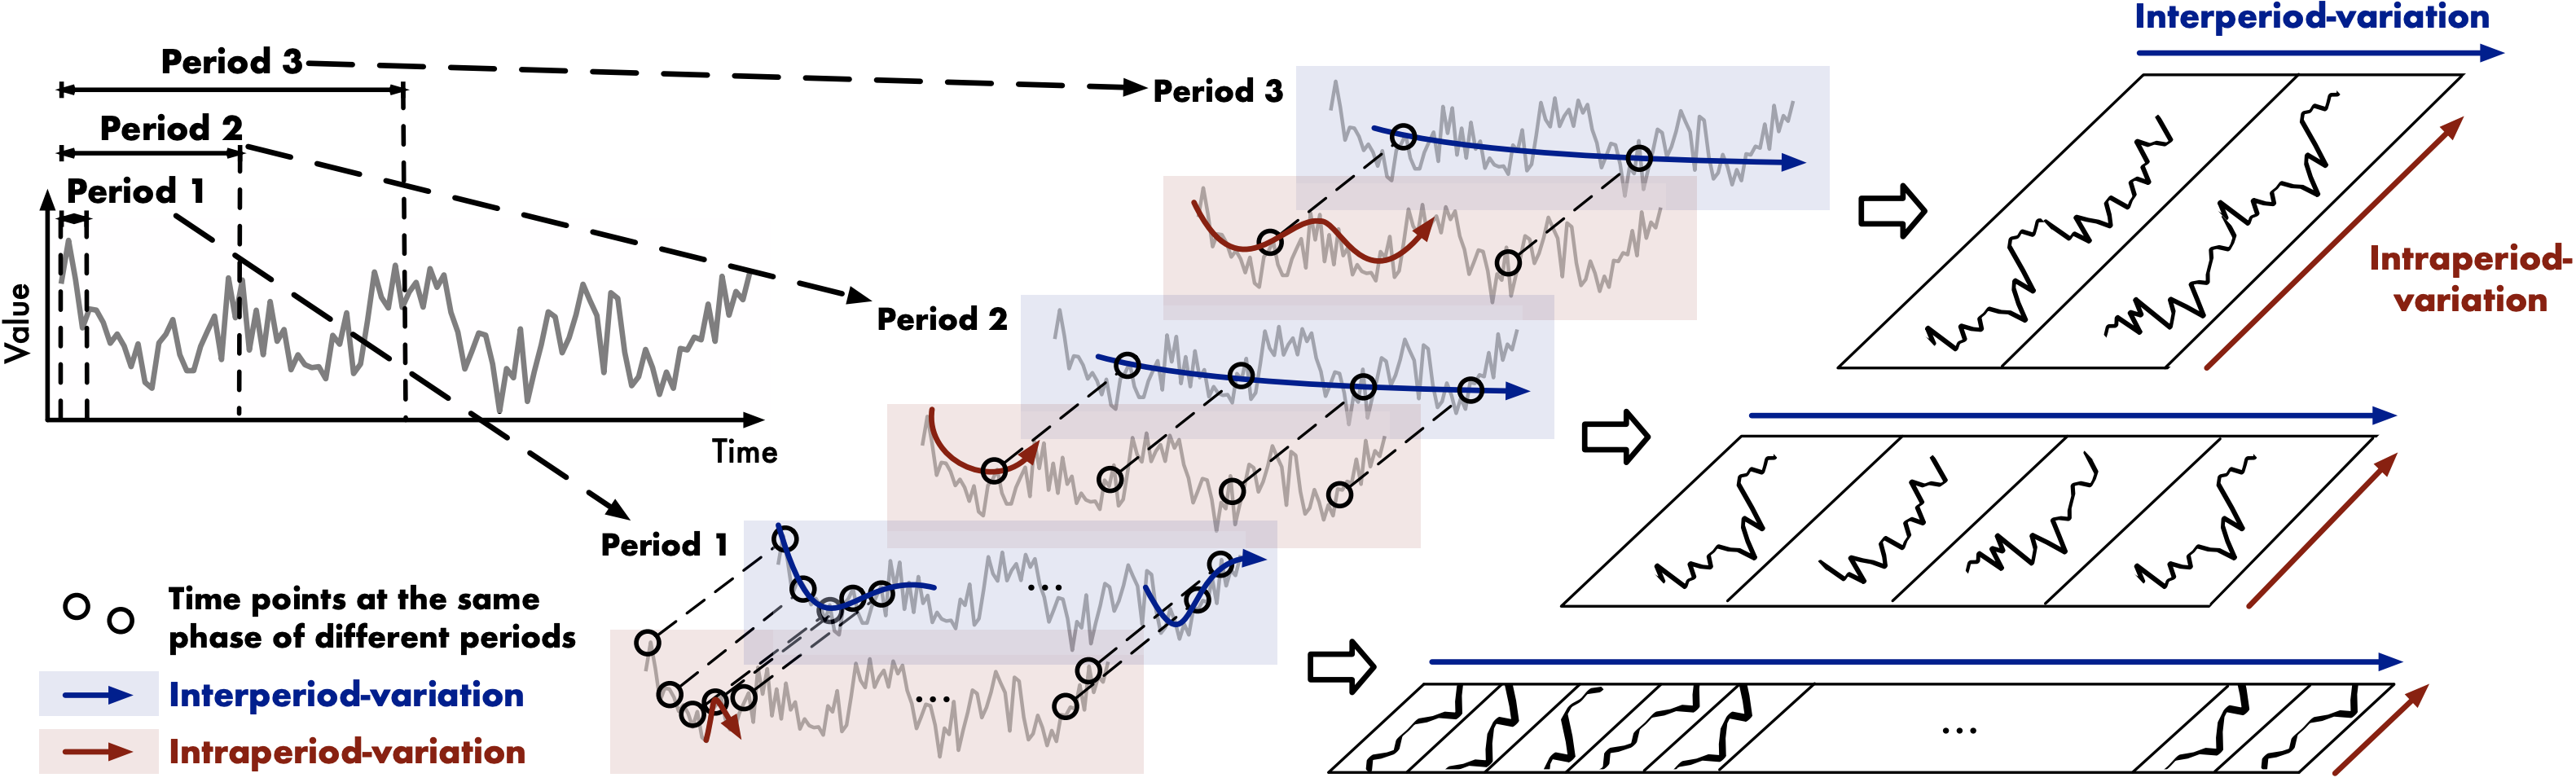
\includegraphics[width=0.4\textwidth]{img/2Dtensor.png}}
\caption{Chuyển đổi chuỗi thời gian 1D ban đầu thành một tập hợp các tensor 2D dựa trên nhiều chu kỳ.}
\label{fig}
\end{figure}